% JCTC (ACS, J. Chem. Theory Comput.) submission build.
% Shared body: paper_body.tex (class-agnostic). Generic/arXiv build: paper_draft.tex.
% Compile: latexmk -pdf paper_jctc.tex   (uses achemso.cls + achemso.bst)
\documentclass[journal=jctcce,manuscript=article]{achemso}
\usepackage[T1]{fontenc}
\usepackage{amsmath,amssymb,amsthm}
\usepackage{graphicx}
\usepackage{booktabs}
\graphicspath{{../figs/}}

\theoremstyle{plain}
\newtheorem{theorem}{Theorem}
\theoremstyle{remark}
\newtheorem*{remark}{Remark}

\DeclareMathOperator{\Var}{Var}
\newcommand{\dF}{\Delta F}
\newcommand{\dFh}{\widehat{\Delta F}}
\newcommand{\ddG}{\Delta\Delta G}

\author{First Author}
\affiliation{Affiliation to be completed}
\email{author@institution.edu}
\title{Read the Uncertainty off the Physics: A Differentiable BAR Bottleneck for Relative
Binding Free Energy, and an Honest Audit of Where Calibration Helps}
\abbreviations{RBFE,BAR,MBAR,FEP}
\keywords{relative binding free energy, Bennett acceptance ratio, uncertainty quantification,
calibration, active learning}

\begin{document}

\begin{tocentry}
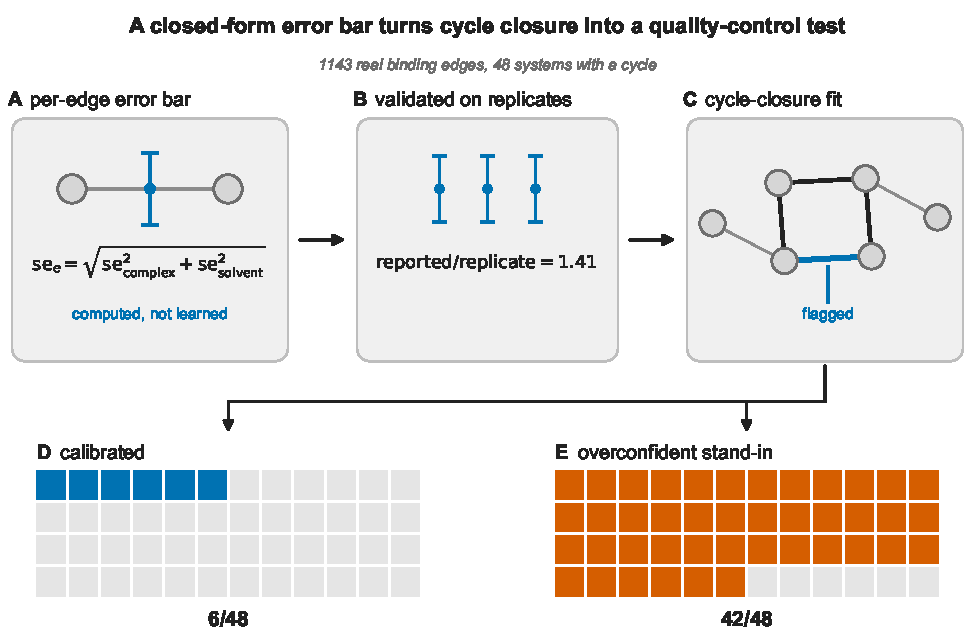
\includegraphics[width=\linewidth]{graphical_abstract.pdf}
\end{tocentry}

\begin{abstract}
A perturbation network's per-edge error splits into two orthogonal parts, and the split decides
what any consistency check can do. One part lives in the network's cycles and can be audited; the
other is a difference of per-ligand offsets and cannot be told from no error at all by any
statistic computed from the network's own values, at any magnitude. The division is unfortunate
rather than neutral: the invisible part is exactly what biases the estimated affinities, and the
auditable part biases nothing. We give the decomposition, the per-edge share of auditability it
implies, and the resolution below which an edge of a planned network can carry no evidence.
Judging the audit quantitatively needs a scale. The Bennett Acceptance Ratio carries its
finite-sampling variance in closed form, and the per-edge error bar a practitioner already
receives is checked here against independent molecular-dynamics replicates on a large set of real
protein-ligand binding edges. Used as the null of a cycle-closure fit it makes the check a test
that flags a selective minority of networks, whose flags reproduce on replicates they never saw,
where an overconfident stand-in flags almost everything. On the public benchmark examined here the
auditable subspace spans a third of the error space, and on systems grounded against public
affinity data it carries under one per cent of the error present. Removing the edges the test
names does not recover accuracy against experiment, nor does removing those a rule derived from
the decomposition prefers. The audit costs nothing beyond the calculation already under way, and
its limits can be stated in advance.
\end{abstract}

\begin{figure}[t]\centering
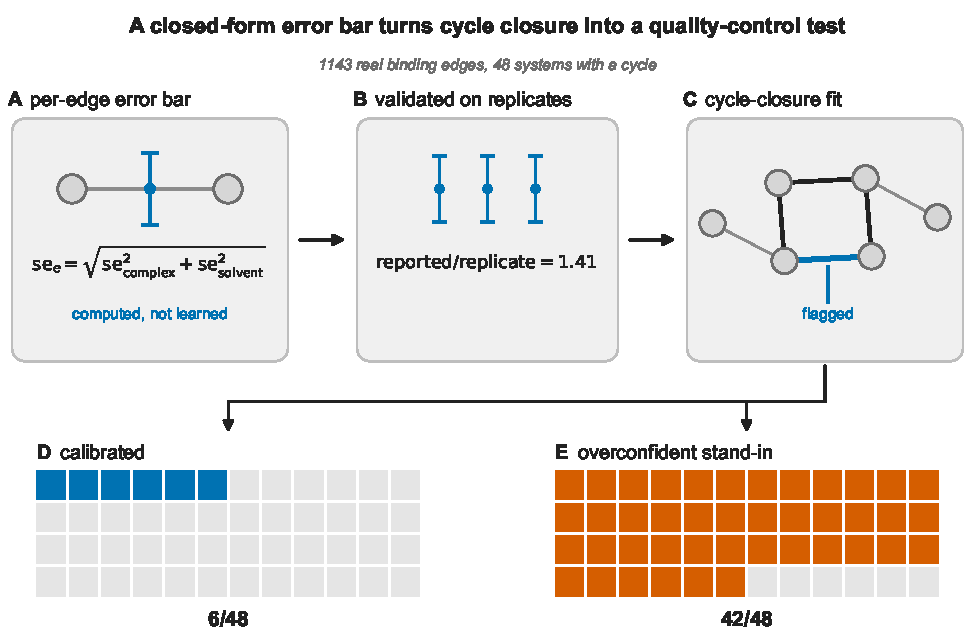
\includegraphics[width=0.96\textwidth]{graphical_abstract.pdf}
\caption{\textbf{Overview.} The pipeline this article runs on the benchmark, left to right. Every
edge arrives with a per-edge standard error the estimator computes rather than learns, composed in
quadrature from the complex-leg and solvent-leg uncertainties; that bar is validated against the
benchmark's three independent protocol repeats (reported over replicate spread $1.41$); and it is
then the null of a generalized-least-squares cycle-closure fit, drawn as a small perturbation
network with one cycle highlighted and one edge marked as flagged. Across the 1143 real binding
edges that lie in the 48 benchmark systems carrying a cycle (of 1145 edges over 49 systems), that
calibrated bar flags 6, 6 and 3 systems on the three repeats, one of them on all three; a stand-in
built edge by edge from a learned head's measured miscalibration profile, not that head run here,
flags 42. The work-sample route to the closed form $B/I^2$ of Theorem~\ref{thm:sand} is deliberately
not drawn: this benchmark releases per-leg uncertainties and no work samples, so that route is
exercised on the alchemtest windows of Figure~\ref{fig:A} and not on these edges.}
\label{fig:overview}
\end{figure}

\section{Introduction}
Relative binding free energy calculations are the most accurate computational tool available for
ranking how tightly a set of candidate molecules will bind a target, and structure-based drug
discovery programs increasingly build them into decisions about which molecules to synthesize.
That accuracy comes at a price: each transformation between two related candidates, one edge of
a perturbation network, requires hours of molecular dynamics simulation, and a realistic project
touches dozens to hundreds of such edges. No program can run every edge to full convergence, so
triage is unavoidable: some edges get simulated first, some get simulated longer, and some
results get trusted enough to act on.

That triage is only as good as the error bar attached to each prediction. A result that looks
converged but is not will silently mislead a ranking of candidates; a result that is genuinely
well converged but reported with an inflated error bar wastes compute chasing a number that was
already trustworthy. A surrogate built to speed up this triage inherits the requirement: every
downstream use of the number, choosing what to simulate next, deciding when to stop, deciding
which candidate to commit to synthesis, consumes the uncertainty as directly as the prediction.

The prevailing way to obtain that uncertainty is to learn it, the same way the prediction itself
is learned: a head trained to output a mean and a variance~\citep{nix1994mve}, an ensemble of
independently trained models whose disagreement stands in for uncertainty~\citep{lakshminarayanan2017ensembles},
or a distribution-free wrapper calibrated after the fact on held-out
data~\citep{angelopoulos2021conformal}. All three treat uncertainty as something to be inferred
statistically from training examples. That approach overlooks a piece of the problem that is
already solved: the estimator that turns raw simulation output into a binding free energy for a
single edge, the Bennett Acceptance Ratio (BAR) estimator~\citep{bennett1976bar}, is a textbook
statistical estimator whose finite-sampling variance has a closed-form expression. That variance
is a property of the estimator, not of the surrogate, and is computed from the same simulation
output that produces the free-energy estimate, with no additional training data.

This work takes that closed form as the uncertainty a screening pipeline should report, and checks
it against independent simulation replicates on a large set of real protein-ligand binding
calculations. What the calibrated bar then buys is a quality-control instrument. A perturbation
network must close its thermodynamic cycles, and how far it fails to close them is already
reported as a diagnostic; fitting that closure against per-edge precisions turns the diagnostic
into a test with a stated null, one that flags networks whose simulations disagree with each other
by more than sampling noise can explain.

The instrument raises a question that has not been asked of the diagnostic it replaces: what can a
cycle see. The answer is a decomposition. Per-edge error decomposes uniquely into a part carried by
the network's cycles and a part that is a difference of per-ligand offsets, the two are orthogonal,
and only the first is identifiable from the network's own values. The second is invisible to every
diagnostic of this kind, at any magnitude, and it is the part that biases the estimated
affinities. That result bounds the instrument, explains which of its uses pay and which do not, and
is measurable: we report how much of the benchmark is auditable, and how much of the error real
networks make against experiment falls where an audit could act on it.

This paper makes the following contributions.
\begin{itemize}
\item A decomposition of a perturbation network's per-edge error into an auditable part carried by
its cycles and a part that is a difference of per-ligand offsets. The second is unidentifiable from
the network's own values at any magnitude, and it is the part that biases the estimated affinities,
while the first biases nothing. The per-edge share of auditability, the shift each edge would need
before a closure test could see it, and the number of absolute measurements needed to resolve the
rest all follow from the same algebra.
\item A measurement of both quantities on a public replicate benchmark. The auditable subspace
spans a third of the error space; on the systems that can be grounded against public affinity data
it carries under one per cent of the error present. Two removal rules fail to improve accuracy
against experiment, the second of them derived from the decomposition itself.
\item A per-edge error bar for a relative binding free energy read off a closed-form expression,
the sandwich variance of the Bennett Acceptance Ratio estimator, rather than learned, and
characterised against independent simulation replicates on real protein-ligand binding data.
\item A quality-control instrument built on that bar. Fitting thermodynamic cycle closure with
calibrated per-edge nulls separates the reproducible part of a network's inconsistency from
ordinary sampling noise, what it identifies reproduces on replicates it never saw, and a bar as
overconfident as a learned one destroys the separation.
\item An applicability map across interval sharpness, edge ranking, synthesis-commit selection
and reward-guided re-ranking, which finds this calibrated uncertainty valuable for detection,
and, in controlled simulation only, for trust in a commit decision and for a
stopping rule; and for nothing sharper or better ranked.
\item The same closed form as an autograd primitive whose backward pass costs a single division,
and as the conductance of a measurement graph whose knowledge gradient is exactly zero along every
gauge-redundant direction.
\end{itemize}

The remainder of this article is organised as follows. Section~\ref{sec:related} places this
work against prior free-energy estimators, learned uncertainty, equivariant trunks, and
acquisition methods. Section~\ref{sec:bar} gives the closed-form sandwich variance and its
replicate validation. Section~\ref{sec:qc} presents the calibrated cycle-closure quality-control
test on real binding data, the decomposition that bounds it, the measurement of where real error
falls against that bound, and what survives a second replicate.
Section~\ref{sec:audit} maps where the calibrated uncertainty helps downstream learning and where
it does not. Section~\ref{sec:methods} gives the data, the estimators, the models and the
simulations behind every number reported above. Section~\ref{sec:limitations} collects the
limitations of the approach, and Section~\ref{sec:conclusion} concludes.

\section{Related work}\label{sec:related}
\paragraph{Free-energy estimators.} BAR~\citep{bennett1976bar} and its multistate
generalization MBAR~\citep{shirts2008mbar} are the standard estimators for alchemical free
energies; FEP+~\citep{wang2015fep} brought them to prospective potency prediction, and large
retrospective assessments~\citep{schindler2020merck} and best-practice guides~\citep{mey2020alchem}
document both their accuracy and their per-edge uncertainty, the sandwich variance of
$M$-estimation~\citep{huber1967,white1982sandwich}.

\paragraph{Learned and recalibrated uncertainty.} The prevailing alternative is to learn
predictive uncertainty: a mean--variance estimation (MVE) head by Gaussian
NLL~\citep{nix1994mve}, a deep
ensemble for the epistemic term~\citep{lakshminarayanan2017ensembles}, the aleatoric/epistemic
split~\citep{kendall2017uncertainties}, or distribution-free conformal
prediction~\citep{angelopoulos2021conformal}, including quantile-adaptive variants such as
CQR~\citep{romano2019cqr}. A predicted $\sigma$ can also be \emph{recalibrated} post hoc by
temperature/Platt scaling~\citep{guo2017calibration} or isotonic
regression~\citep{zadrozny2002isotonic}.

\paragraph{Equivariant trunks and chirality.} $E(3)$-equivariant
networks~\citep{geiger2022e3nn,batzner2022nequip,batatia2022mace} are the de-facto trunks for
3D molecular property prediction, and the use of parity-\emph{odd} (pseudoscalar) irreps to
break achirality is standard in that literature.

\paragraph{Acquisition and reward re-ranking.} Acquisition by the knowledge gradient~\citep{frazier2008kg}
and its Monte-Carlo implementations~\citep{balandat2020botorch,gardner2018gpytorch} drive edge
selection, while GFlowNets~\citep{bengio2021gflownet,malkin2022tb} sample candidates in
proportion to reward; the resistance distance of a weighted graph Laplacian equals contrast
variance in a Gaussian graphical model~\citep{klein1993resistance}.

The works cited above use that uncertainty as a reported number or as a separately learned model.
This work characterises the same sandwich variance against independent replicates, puts it to a
distinct use as the calibrated null of a real-data cycle-closure quality-control test, and
supplies it as a differentiable quantity that is also the conductance of a gauge-aware acquisition graph.

\section{The per-edge error bar}\label{sec:bar}
\paragraph{Setup.} For a single alchemical edge, forward and reverse works
$\{W^f_i\}_{i=1}^{n_f}$, $\{W^r_j\}_{j=1}^{n_r}$ define unified coordinates $x_i=W^f_i$,
$x_j=-W^r_j$. With $M=\ln(n_f/n_r)$ and $p(x;d)=s(x-d+M)$ (here $s(\cdot)$ is the logistic
function, distinct from the uncertainty $\sigma$ used later), the
BAR estimate $\dFh$ is the
root of the score $S(d)=\sum_{j\in r}p(x_j)-\sum_{i\in f}(1-p(x_i))$, and
$\partial_d S=-\sum p(1-p)=:-I(d)$, the curvature/overlap.

\begin{theorem}[$O(1)$ differentiable backward]\label{thm:back}
Let $\dFh(\theta)$ be defined by $S(\dFh,\theta)=0$ with non-degenerate curvature $I\neq0$
(positive overlap). The implicit function theorem gives $d\dFh/d\theta=I^{-1}\partial_\theta S$.
For window means, $d\dFh/d\mu^f=I^f/I$, $d\dFh/d\mu^r=-I^r/I$, with $|I^f/I|+|I^r/I|=1$. The
backward pass is one division by the curvature; the root-find is not unrolled.
\end{theorem}
Theorem~\ref{thm:back} is a statement about cost, and cost is the whole of the role the
differentiable layer plays here: it prices carrying the bar inside a model at one division per
backward pass, with the root-find not unrolled. No experiment reported below trains through the
layer. Everything below consumes the variance as a number or as a fixed graph weight.

\begin{theorem}[Sampling variance via the sandwich]\label{thm:sand}
$\dFh$ is an $M$-estimator; its asymptotic sampling variance is the sandwich
$\Var(\dFh)=A^{-1}BA^{-1}=B/I^2$, with $A=I$ and $B=n_f\Var_f[p]+n_r\Var_r[p]$
\citep{huber1967}. Here $A\neq B$ arises from BAR's \emph{stratified two-sample design}, not
from model misspecification; the sandwich is the sample-computable form and agrees with the
Bennett/Shirts--Chodera (MBAR) uncertainty
\citep{bennett1976bar,shirts2008mbar}. Concretely, the plug-in MBAR/Bennett uncertainty is
$\Var_{\text{MBAR}}=1/I-(1/n_f+1/n_r)$ (identical to \texttt{pymbar}'s \texttt{MBAR}
uncertainty). Evaluated at the root, with works drawn from the correct pair of ensembles, this
is not an approximation to the sandwich but the same quantity: $B/I^2=1/I-(1/n_f+1/n_r)$
identically, so the $-(1/n_f+1/n_r)$ term is precisely the $O(1/n)$ gap between the naive
information-equality plug-in $1/I$ and the sandwich. The two \emph{sample} plug-ins differ only
through the moments they substitute, and that difference shrinks with $n$ (paired
Monte-Carlo check against the released implementation: the
mean paired $|\Var_{\text{MBAR}}-B/I^2|$ falls monotonically and by more than an order of
magnitude from $n{=}40$ to $n{=}320$, the range this repo verifies; beyond that the paired
discrepancy is smaller than Monte-Carlo noise at a modest replicate budget, so we do not quote
a range past $320$). This is why bare $1/I$ (Figure~\ref{fig:A},
naive) overstates the calibrated uncertainty and \texttt{pymbar}'s reported MBAR se does not.
\end{theorem}

\begin{remark}[scope of ``calibrated'']
$B/I^2$ is the variance of the \emph{sampling} error of $\dFh$, conditional on the works being
drawn from the correct alchemical ensembles. It says nothing about systematic force-field bias,
which is outside $B/I^2$ (we attach a separate epistemic/correction term in
Section~\ref{sec:audit}). The value of Theorem~\ref{thm:sand} for us is that this term is a
differentiable closed form (Theorem~\ref{thm:back}) and is non-negative by construction, where
the plug-in MBAR expression can return a negative value in a rare edge case
(very high overlap with tiny samples, where the plug-in $1/I$ undershoots the
$1/n_f+1/n_r$ correction), whereas $B/I^2\ge0$ always.
\end{remark}

The information equality $A=B$ (which would give $1/I$) holds for a single-sample MLE but fails
for BAR's two-sample design; we verify the gradients to machine precision and the variance to
within $1\%$ against $3000$-replicate Monte-Carlo and \texttt{pymbar} in the good-overlap
regime (at extreme low overlap, $n{=}20$, the bias-corrected plug-in runs $\sim$10\% below
MBAR, both $\approx1$).
The sandwich is derived for independent samples; on real FEP works both the sandwich inputs and the bootstrap truth are subsampled to the statistical inefficiency $g$~\citep{shirts2008mbar} before $B$ is formed, so the reported panel-B ratios use effective $n$.

\paragraph{Figure~\ref{fig:A}: the readout is correct; the learned foil is not.}
Figure~\ref{fig:A}A sweeps the work-distribution overlap. The sandwich $B/I^2$ coincides with MBAR
and Monte-Carlo truth across the range (reported/true se $\approx1$), with no Monte-Carlo. A
\emph{fair} learned mean--variance head, trained by Gaussian NLL on work-summary moments
\emph{and} the overlap scalar $I$, is ${\approx}7\times$ overconfident at a realistic budget of
$\sim$$200$ edges (reported se ${\approx}0.15\times$ the truth, range $0.09$--$0.20\times$) and
${\approx}5\times$ overconfident at a twenty-fold larger oracle budget. A seed sweep and two
corrected foils leave that unchanged: an objective fix does not recover calibration and an
ensemble is unreliable in both directions at this budget (Supporting Information). The residual
overconfidence is a \emph{data-efficiency} limit of a learned per-edge variance rather than an
identifiability barrier or an artifact of the Gaussian-NLL objective, and the bottleneck
\emph{computes} the variance exactly at zero label cost, so the comparison is learnable-with-data
against exact-and-free. Bare $1/I$ appears only as the information-equality plug-in it corrects
($1.08$--$2.65\times$, worst at high overlap), not as a baseline anyone reports.
Figure~\ref{fig:A}B checks the same calibration on work samples from a real protein--ligand
system, the $19$ adjacent-$\lambda$ BAR windows of the complex leg of the \texttt{alchemtest} BACE1
relative-binding calculation (sandwich over decorrelated-bootstrap truth $1.00$, $[0.96,1.07]$;
naive $1/I$ over the same reference $2$--$12\times$, mean $6.07$, every window at overlap
$\geq0.84$; per-window values, Supplementary Table~\ref{tab:bace1}). That reference reuses the same
work samples, so the panel establishes agreement with a decorrelated bootstrap on real molecular
dynamics in the high-overlap regime this schedule occupies, not a ligand-to-ligand binding
quantity; the low-overlap behaviour is the controlled sweep of panel A and the per-transformation
quantity is Figure~\ref{fig:Arep}.

\paragraph{Figure~\ref{fig:Arep}: the reported bar against independent replicates.} The
validation that does not reuse its own samples, and the result the detector of
Section~\ref{sec:qc} rests on, is Figure~\ref{fig:Arep}. Each edge's reported bar
is composed in quadrature from the complex-leg and solvent-leg MBAR uncertainties shipped with
the benchmark, $\mathrm{se}=\sqrt{\mathrm{se}_{\text{complex}}^2+\mathrm{se}_{\text{solvent}}^2}$;
each leg term is a multistate MBAR uncertainty over that leg's $\lambda$ windows, not the
two-state BAR quantity of Theorem~\ref{thm:sand}, so what is validated here is the bar as a
practitioner receives it rather than the two-state identity itself. Across $1145$ real
binding edges from
the OpenFE IndustryBenchmarks2024~\citep{baumann2025industrybenchmarks} (3 independent replicates
each), the reported MBAR se is calibrated-to-conservative against the across-replicate
truth (reported/replicate-SD $1.41$, CI $[1.26,1.62]$; conservative on $72\%$
of edges and on $28$ of the $34$ systems carrying at least eight edges). Both sides of that ratio pool in quadrature, so the
$n{=}3$ replicate term is unbiased at the variance level and needs no small-sample
correction.
The three replicates are independent stochastic repeats of the sampling process from identical
starting coordinates (OpenFE \texttt{protocol\_repeats}~\citep{baumann2025industrybenchmarks});
the across-replicate SD therefore reflects sampling/convergence noise alone and is a
\emph{lower bound} on full reproducibility (it excludes pose and system-preparation variance).
The reported se does not \emph{systematically} under-state real
reproducibility, the opposite of the learned head's ${\approx}7\times$ overconfidence
at realistic budget (${\approx}5\times$ even at large budget).

That conclusion points the other way from the closest measurement in the literature.
\citet{wade2022estimators} compare the analytic MBAR uncertainty against the spread over five
independent replicas on $54$ protein-ligand transformations across five targets, in two engines,
and report that MBAR consistently \emph{under}-estimates the error, by up to $0.9$ kcal/mol. Two
differences bear on the disagreement and they point opposite ways. Their replicas resample the
full ensemble, whereas the OpenFE repeats share starting coordinates, so our denominator is a
lower bound on run-to-run variability and our ratio an upper bound on conservatism. But running
their own functional on these edges sharpens the disagreement rather than resolving it: the
analytic standard error falls below the replicate spread on $0.279$ $[0.224,0.332]$ of edges,
against the $0.368$ correctly scaled bars produce at three replicates, and the interval excludes
it. Settling the question needs replicates that resample preparation and pose, which this
benchmark does not provide.

\begin{figure}[t]\centering
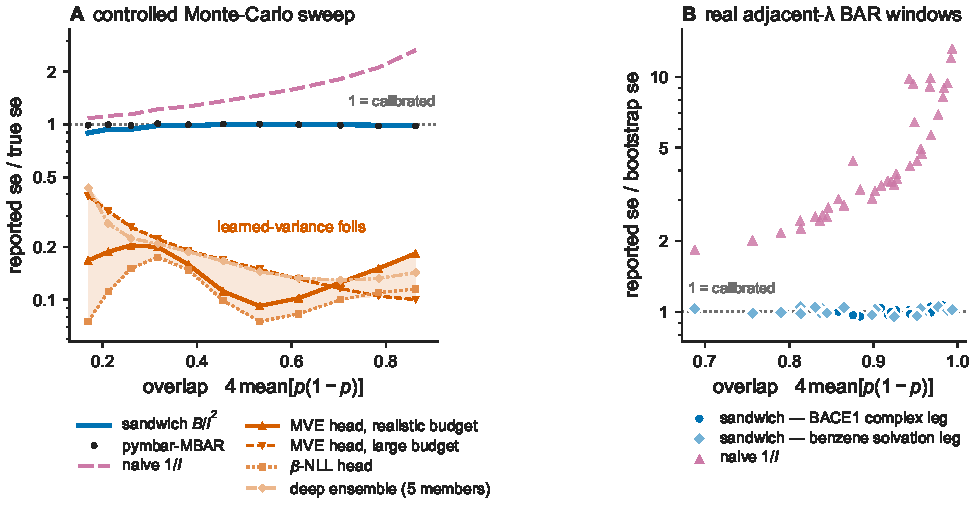
\includegraphics[width=0.92\textwidth]{figA_target_the_sandwich.pdf}
\caption{\textbf{Sandwich variance against learned-variance foils, controlled and real data.}
(A) Reported standard error divided by the true standard error, versus work-distribution
overlap, for the sandwich $B/I^2$, \texttt{pymbar}-MBAR, the naive information-equality
plug-in $1/I$, a learned mean--variance (MVE) head at a realistic and at a large training
budget, a $\beta$-NLL head, and a $5$-member deep ensemble, in a controlled Monte-Carlo
sweep.
(B) Reported standard error versus decorrelated-bootstrap standard error on the $19$
adjacent-$\lambda$ BAR windows of the complex leg of the \texttt{alchemtest} BACE1
relative-binding calculation (filled circles) and on the $19$ windows of the benzene solvation
legs (filled diamonds), for the sandwich
$B/I^2$ and the naive $1/I$. Each point is one two-state BAR estimate between neighbouring
$\lambda$ values, not a ligand-to-ligand binding free energy.}
\label{fig:A}
\end{figure}

\begin{figure}[t]\centering
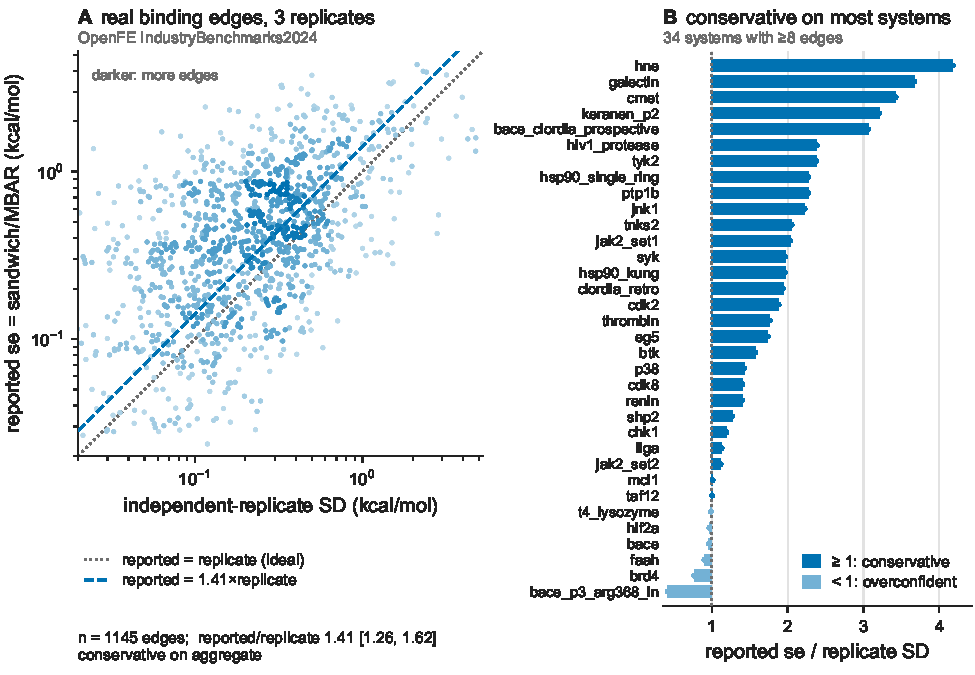
\includegraphics[width=0.92\textwidth]{figA_replicate_validation.pdf}
\caption{\textbf{Independent-replicate validation on real binding edges.} Reported
per-edge standard error versus the across-replicate empirical standard deviation, on
$1145$ OpenFE IndustryBenchmarks2024~\citep{baumann2025industrybenchmarks} edges (3
independent replicates each). (A) Reported standard error versus across-replicate
standard deviation, with the $y{=}x$ line. (B) Per-system pooled ratio of reported
standard error to across-replicate standard deviation, for the $34$ benchmark systems carrying at
least eight edges (Section~\ref{sec:methods}). These are systems, not distinct proteins:
\texttt{jak2\_set1} and \texttt{jak2\_set2}, and \texttt{hsp90\_single\_ring} and
\texttt{hsp90\_kung}, are separate systems of the same protein.}
\label{fig:Arep}
\end{figure}

\begin{theorem}[Fisher--resistance correspondence]\label{thm:fr}
For relative measurements $y_e=(\varphi_j-\varphi_i)+\varepsilon_e$,
$\varepsilon_e\sim\mathcal N(0,V_e^{\mathrm{true}})$ with $V_e^{\mathrm{true}}=B_e/I_e^2$, the
Gaussian posterior precision of
the node potentials is the weighted Laplacian $L=\sum_e w_e(e_i-e_j)(e_i-e_j)^\top$ with
conductances $w_e=1/V_e^{\mathrm{true}}=I_e^2/B_e$. Contrast variance equals effective
resistance~\citep{klein1993resistance}, a single edge recovers $V_e^{\mathrm{true}}$,
Sherman--Morrison gives
$O(1)$ acquisition updates, and $\ker L\supseteq\mathrm{span}\{\mathbf 1\}$, so the knowledge
gradient (KG)~\citep{frazier2008kg} is exactly zero on gauge/redundant directions: the acquisition is
automatically gauge-invariant.
\end{theorem}
The edge weights are the inverse sandwich variances, the readout of Section~\ref{sec:bar}
entering the decision layer; the acquisition model identifies the reported variance with the true
one ($c_e=1$), which is the assumption the replicate validation of Section~\ref{sec:bar} tests
rather than one this section adds. The gauge-zero property is structural: KG$=0$ on gauge directions
follows from the kernel inclusion alone, so it does not depend on the weight \emph{value}, and by
Gauss--Markov the value does not improve ranking (Section~\ref{sec:audit}). For a \emph{connected}
network the inclusion is an equality, $\ker L=\mathrm{span}\{\mathbf 1\}$, for any positive
conductances, and the overall additive offset is then the only unidentifiable direction; a network
with $k$ components has a $k$-dimensional kernel, one offset per component. The
Laplacian-precision and resistance-distance machinery is classical generalized least squares (GLS)
on graphs and the resistance distance of \citet{klein1993resistance}; what is specific here is the
\emph{sandwich} precision $I_e^2/B_e$ as the conductance, not raw overlap, and the automatic
gauge-invariance of the acquisition.

\section{Calibrated cycle-closure quality control}\label{sec:qc}
The capability this paper demonstrates is the separation of the \emph{reproducible} part of a
perturbation network's edge-level inconsistency from its \emph{sampling noise}, using the bar of
Section~\ref{sec:bar} as the null of a quality-control (QC) test. The candidate physical sources of
a reproducible part are the usual ones, non-convergence, hysteresis, and charge, water or
protonation artifacts, but this design does not identify which of them is present, and it does not
separate them from a fixed consequence of the one starting structure every repeat begins from. The
calibration underwriting the null is
validated against seed and velocity replicate spread, a lower bound on full run-to-run
reproducibility (it excludes pose and system-preparation variance), and the same restriction bounds
what the detection claims below can mean: an inconsistency that survives repeats sharing their
starting coordinates is established as more than sampling noise, not as physical error. This is \emph{detection}, not weighting of a fixed
estimate: the Gauss--Markov ceiling that makes the calibrated variance second-order elsewhere (in a
connected graph the GLS contrast mean is unbiased for \emph{any} positive weights, so the weight
\emph{value} cannot improve ranking, Section~\ref{sec:audit})
does not bind a goodness-of-fit test, whose statistic depends on the weights directly.

\paragraph{A calibrated cycle-closure test.} A perturbation network must close its cycles: the
signed sum of $\ddG$ around any loop is zero in expectation. Fitting node potentials by
generalized least squares with conductances $w_e=1/V_e^{\mathrm{rep}}$, which
Theorem~\ref{thm:fr} identifies
with the sandwich precision $I_e^2/B_e$ whenever the work samples are available (on this benchmark
they are not released, so $V_e^{\mathrm{rep}}$ is the reported per-edge variance composed from the
two legs, Section~\ref{sec:methods}),
gives residuals $r_e$ and the goodness-of-fit statistic
$X^2=\sum_e r_e^2/V_e^{\mathrm{rep}}\sim\chi^2(\mathrm{dof})$,
with $\mathrm{dof}$ the number of independent cycles ($E$ minus the incidence rank). Under
correctly-sampled physics $\mathbb{E}[X^2/\mathrm{dof}]\approx1$; here it runs \emph{below} one
(median $0.34$), qualitatively consistent with the conservative bars of Figure~\ref{fig:Arep}.
We do not convert that median into a conservatism factor. The quantity the closure statistic
identifies is not a median. Two variances have to be told apart from here on: the variance a
practitioner is handed, $V_e^{\mathrm{rep}}$, which is what the fit uses as its weight, and the
variance the edge actually has, $V_e^{\mathrm{true}}$. They are related by
$V_e^{\mathrm{rep}}=c_e^2V_e^{\mathrm{true}}$, so the per-edge calibration ratio $c_e$ is the
reported standard error over the true one: $c_e>1$ is a reported bar that is too wide
(conservative) and $c_e<1$ one that is too tight (overconfident), and $c_e$ is measured on this
benchmark as the reported standard error over the across-replicate standard deviation. Whitening
by the reported errors gives $\mathbb{E}[X^2]=\operatorname{tr}(\Pi D)$ with
$D=\mathrm{diag}(c_e^{-2})$,
so, as Theorem~\ref{thm:cons} below establishes, $\mathbb{E}[\chi^2_\nu]$ is the curl-leverage-weighted \emph{mean} of $c_e^{-2}$. Inverting a median recovers a scalar conservatism only when $c_e$ is constant across
edges, and Figure~\ref{fig:Arep}B shows it is not. A replicate-validated ratio and a
closure-implied one are therefore different functionals of a heavy-tailed per-edge ratio
distribution, and no single scalar conservatism factor is identified by these data; the apparent
disagreement between them is an artefact of comparing different functionals rather than a physical
discrepancy. Residual correlation among edges sharing a ligand endpoint, which the diagonal-$V$ GLS
does not model, is separately negligible (excess correlation over the projector-induced
null $-0.0079$ $[-0.0314,+0.0164]$). The Benjamini--Hochberg flag set is unchanged. A reduced
$\chi^2$ well above one signals edge-level inconsistency in excess of sampling noise. The test is
(correctly) blind to node-consistent force-field bias, which cancels around a loop.

\begin{theorem}[Estimation--detection conservation law]\label{thm:cons}
In the whitened GLS fit let $\Pi=\mathbb{I}-H$ be the residual-maker projector onto the cycle
space ($\Pi$, to keep $M$ for the log sample-size ratio of Section~\ref{sec:bar} and $R$ for a
Pearson correlation). Its diagonal, the curl-leverage $h_e=\Pi_{ee}$, satisfies $h_e+w_e\Omega_e=1$ with
$w_e=1/V_e^{\mathrm{rep}}$ and
$\Omega_e$ the effective resistance of edge $e$ (Theorem~\ref{thm:fr}); hence
$\sum_e h_e=\mathrm{dof}$, and the closure-$\chi^2$ noncentrality against a systematic shift $\mu$
on edge $e$ is $h_e\mu^2/V_e^{\mathrm{rep}}$. A bridge edge (in no cycle) has $h_e=0$ and is
undetectable at any
$\mu$; a node-consistent (gradient) bias lies in $\mathrm{range}(H)$ and is annihilated by $\Pi$.
The QC's blindness to node-consistent force-field bias is therefore a \emph{derived} property, not
an assumption, and $h_e$ is a per-edge observability certificate with detectable-shift resolution
$\delta^\ast_e=\sqrt{V_e^{\mathrm{rep}}/h_e}$.
\end{theorem}
The algebra is standard and we claim none of it: $h_e=\Pi_{ee}$ is the hat-matrix leverage of the
whitened design, its complement $w_e\Omega_e$ is the classical correspondence between leverage and
effective resistance~\citep{klein1993resistance}, and $\sum_e h_e=\operatorname{tr}(I-H)=\mathrm{dof}$
is the trace identity for a projector. What the theorem adds is the reading of $h_e$ as a per-edge
observability certificate, which turns the test's blindness to node-consistent bias from a
modelling assumption into a consequence and names, before any simulation is run, the edges that
can carry no evidence at all.
The resulting map lists the structurally un-auditable (bridge) edges per system; on this benchmark the
curl-leverage does not additionally predict the \emph{location} of reproducible systematic error
(studentized Spearman $\rho=-0.073$, permutation $p=0.9571$, not significant; Supplementary
Figure~\ref{fig:Lev}), so we claim only the structural certificate.

Theorem~\ref{thm:cons} is the diagonal of a statement about the whole error space, and the whole
statement is what bounds the method. Write the per-edge systematic error as a vector $\mu$ over the
$E$ edges. Whitening and projecting splits it, orthogonally and uniquely, into a part that lies in
the cycle space and a part that is a difference of per-ligand offsets.

\begin{theorem}[Auditable and unauditable error]\label{thm:hodge}
In the model $y=A\varphi+\mu+\varepsilon$ with $A$ the signed incidence matrix of a network of $N$
ligands, $E$ edges and $c$ components, and $\varphi$ unknown:
\emph{(i)} for every $\delta$, the parameter pairs $(\varphi,\mu)$ and $(\varphi+\delta,\mu-A\delta)$
induce the same distribution of $y$, so $\mu$ is identifiable only through $\Pi\tilde\mu$. The
auditable subspace has dimension $\mathrm{dof}=E-N+c$ and its orthogonal complement, the gradient
fields $\mu_e=b_j-b_i$, has dimension $N-c$ and is unidentifiable: no statistic computed from a
network's own edge values distinguishes a per-ligand bias from no bias, at any magnitude.
\emph{(ii)} The bias such an error induces in the fitted potentials, $(\tilde A^\top\tilde
A)^{+}\tilde A^\top\tilde\mu$, depends only on the gradient part, while the closure noncentrality
$\|\Pi\tilde\mu\|^2$ depends only on the cycle part. What the test can see and what corrupts the
answer are exact orthogonal complements.
\emph{(iii)} For an error field with no preferential alignment, the expected visible fraction
$\|\Pi\tilde\mu\|^2/\|\tilde\mu\|^2$ is $\mathrm{dof}/E$.
\emph{(iv)} Given absolute measurements on a set $S$ of ligands, the unidentifiable dimension is
$(N-|S|)-c_{\mathrm{free}}(S)$, with $c_{\mathrm{free}}$ the number of components holding none of
them: the first anchor in a component removes only that component's arbitrary offset and buys no
identifiability, each further anchor buys exactly one dimension, and resolving a per-ligand bias in
full requires an absolute measurement on every ligand.
\end{theorem}
The decomposition is the two-term discrete Hodge splitting of an edge field into gradient and cycle
parts; splitting the cycle space further into curl and harmonic components would require a choice
of two-cells and is not needed here. Part (i) is the reparametrisation invariance of the model and
part (iii) is $\operatorname{tr}(\Pi)/E$. What the theorem contributes is not the algebra but its
reach: the blindness is a property of the data rather than of one statistic, so it binds fixed
hysteresis cutoffs, weighted cycle closure and any future closure-based diagnostic alike, and part
(ii) says that blindness is aligned with harm rather than incidental to it.

Network maximum-likelihood
estimation of $\ddG$ networks~\citep{xu2019diffnet}, cycle-closure hysteresis as a
diagnostic~\citep{wang2015fep,cui2020hysteresis}, weighted cycle closure~\citep{li2023wcc}, and the
constrained variational solution of a whole network under loop closure~\citep{giese2021variational}
are established; what is new is the \emph{calibrated} null: a
per-edge, replicate-validated aleatoric variance that gives the test per-edge-adaptive thresholds
and a false-positive rate controlled \emph{to the extent the per-edge null is calibrated}
(validated against independent replicates, Figure~\ref{fig:Arep}), complementing the field's fixed
hysteresis cutoffs, together with the cross-replicate reproduction check of Figure~\ref{fig:Lval}B and the
estimation--detection conservation law of Theorem~\ref{thm:cons}, which fixes which edges are
auditable at all; what is shared with the works above is the weighted least-squares treatment of the
cycle graph itself. On the same $1143$ edges a pre-registered head-to-head scored the calibrated per-edge null against
the fixed $1.0$ kcal/mol hysteresis cutoff the field uses and against a fixed-$\mathrm{se}$
$\chi^2$ test, by area under the receiver-operating-characteristic curve; the criterion required
beating both, and the verdict was a tie (Supplementary Figure~\ref{fig:Cut}). We withdraw the
further reading we placed on the ordering inside it. The only label these data supply divides each
residual by the same per-edge variance the calibrated rule uses as its weight, so the ordering is
monotone in proximity to that variance rather than in detection skill, and the comparison ranks
nothing. What the calibrated null has over a fixed cutoff is accordingly structural: per-edge
adaptive thresholds, a false-positive rate tied to a replicate-validated null, and the
observability map of Theorem~\ref{thm:cons}. The evidence that the flags are real remains the
distribution-free cross-replicate reproduction check, which does not depend on the $\chi^2$
scaling, and it needs only the per-edge $se$ the benchmark ships: the detector's novelty is the
calibrated null, not the differentiable machinery.
That null is conservative in the bulk, with a median reduced $\chi^2$ of $0.34$, so on a typical system the test under-flags.
That observation does not bound the realized false-positive rate, and we do not read it as doing
so: Benjamini--Hochberg controls the false discovery rate through the behaviour of the null
$p$-values near the rejection threshold, not through the median of the statistic, and the
per-system calibration of Figure~\ref{fig:Arep} is heterogeneous enough that a conservative bulk
and an anti-conservative tail can coexist. The nominal level is reported as nominal. The case for
the flags therefore rests not on the $\chi^2$ tail but on the
distribution-free cross-replicate reproduction check below,
which assumes no Gaussian null. A subtler concern is that four of the six flagged systems are themselves locally overconfident
against their own across-replicate spread (Figure~\ref{fig:Arep}: \texttt{brd4} $0.76\times$,
\texttt{faah} $0.90\times$, \texttt{bace} and \texttt{hif2a} $0.96\times$), so a flag could partly
reflect that system's own too-tight bars. Retesting each against the width its own replicates
measure keeps all six at the per-system granularity and \emph{two} of them, \texttt{bace} and
\texttt{cdk8}, at the per-edge granularity this work pre-specified. Supplementary
Table~\ref{tab:selfgrid} reports both arms with their two-sided counterparts and each arm's
realized false-flag probability under the pure-null simulation of Section~\ref{sec:methods}; the
pre-specified per-edge one-sided arm is the only self-calibrated arm that holds its level ($0.003$
against a nominal $0.05$), so its count of two is the conservative answer.

\paragraph{Figure~\ref{fig:L}: a deployable detector whose usefulness \emph{is} $\sigma$-calibration.}
On the OpenFE IndustryBenchmarks2024~\citep{baumann2025industrybenchmarks} ($1145$ edges over
$49$ systems, of which the $48$ with $\geq1$ independent cycle, holding $1143$ edges, admit the
test; $3$ replicates), the median reduced
$\chi^2$ is $0.34$ and a Benjamini--Hochberg false-discovery-rate (FDR)
test at $0.05$ applied to the first replicate flags six chemically-sensible systems
(\texttt{brd4}, \texttt{bace}, \texttt{faah},
\texttt{cdk8}, \texttt{hif2a}, \texttt{p38}; Figure~\ref{fig:L}A; \texttt{brd4}'s data set is a
buried-water set, \texttt{bace} is protonation-sensitive). That particular set of six is a
single-replicate draw and should not be read as a census; Section~\ref{sec:stability} measures how
much of it survives the other two replicates. Supplementary Tables~\ref{tab:stab}
and~\ref{tab:stab2} report, for all $48$ systems and each replicate separately, the degrees of
freedom, the reduced $\chi^2$, and the Benjamini--Hochberg adjusted $q$-value behind every flag.
The detector's value is entirely a
function of calibration (Figure~\ref{fig:L}B): a uniform ${\times}0.15$ shrink standing in for the
learned head's central overconfidence (Figure~\ref{fig:A}) flags $88\%$ of systems ($42$ of
$48$), which leaves almost nothing unflagged and so no longer separates anything, the calibrated
sandwich flags $12\%$ ($6$ of $48$, selective), a $\times1.3$ inflation one system of $48$, and a
$\times2$ inflation none. We report these as flagged fractions rather than as false-positive
rates: which of the flags are false is exactly what is not known here
(Section~\ref{sec:limitations}).

The count is not separable from the level, and the level moves first. The scale at which the
reported bars are correct follows from the functional that governs the statistic rather than
from a pooled ratio: the curl-leverage-weighted mean of $c_e^{-2}$ is $0.853$, so the bars are
wide by $1.08\times$ and the calibrated scale is $0.92$, with the bootstrap interval on that mean
putting it in $[0.79,1.04]$. Across that interval the flag count runs from six to nine. But under
a simulation in which the reported bar is correct by construction, the probability that the test
flags anything at all is $0.043$ at scale $1.00$, $0.237$ at $0.92$ and $0.933$ at $0.79$: a
tightening of eight per cent costs the level a factor of five, and one of twenty per cent
destroys it. Only the top of the calibration interval is an operating point at which the test
controls what it claims to control, which is why the six systems are quoted there and why a
larger count obtained by tightening the bars is not a more sensitive setting but a less valid
one. That
uniform shrink is a stress test rather than a realistic head. Applying instead the learned head's
\emph{measured}, overlap-dependent miscalibration profile per edge (rank-transferred onto each
edge's own overlap, Supplementary Figure~\ref{fig:P4}) flags $42$ of $48$ systems against the
calibrated sandwich's $6$ ($7.00\times$), so the degradation survives a heterogeneous, non-uniform
profile and is not an artifact of the uniform factor. A shuffled-profile control and a swept
shrink magnitude (Supplementary Figure~\ref{fig:P4b}) place the same reading on it: it is
the \emph{magnitude} of the learned head's miscalibration, not the \emph{uniformity} of
the Figure~\ref{fig:L}B stand-in, that destroys the test, over-wide bars cost power in the other
direction, and the calibrated scale is a two-sided optimum rather than a plateau. The
demonstration is accordingly scoped to heads as overconfident as the measured one (reported
$\mathrm{se}$ $5$--$11\times$ too small); it establishes that such heads saturate the test, not the
shrink magnitude at which selectivity is first lost. The
three independent replicates confirm the flagged inconsistency is reproducible rather than
sampling: pooling the
replicates shrinks the bars ($\mathrm{se}\to\mathrm{se}/\sqrt3$) yet \emph{increases} the flagged
systems' reduced $\chi^2$ toward the $3\times$ variance-components ceiling (Figure~\ref{fig:L}C),
which occurs only for a component that repeats (single-replicate
$\chi^2_\nu=1+\sigma^2_{\text{sys}}/V_{\text{samp}}$ vs
pooled $1+3\sigma^2_{\text{sys}}/V_{\text{samp}}$, with $\sigma^2_{\text{sys}}$ the reproducible
variance component and $V_{\text{samp}}$ the sampling one; the ratio $\to3$ iff
reproducible-dominated). The argument fixes the component's variance, not its origin. It is
invariant to whether $\sigma^2_{\text{sys}}$ is physical error or a fixed consequence of the one
starting structure the three repeats share, because both are constant across repeats and both
therefore survive the average the same way.

\begin{figure}[t]\centering
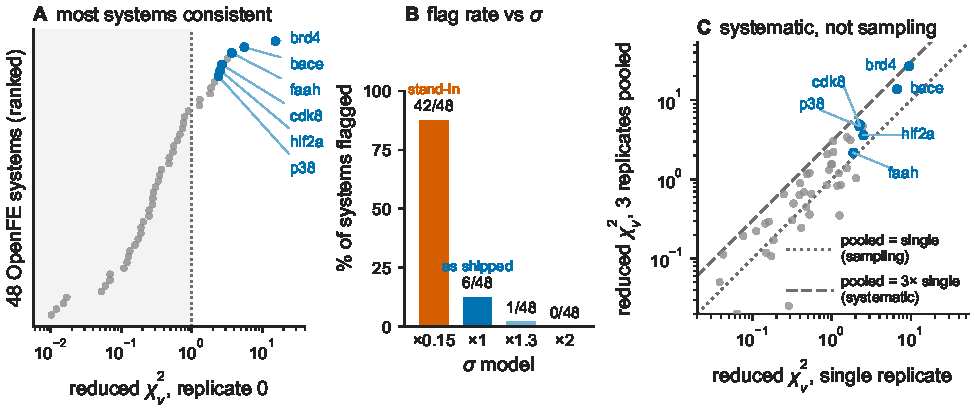
\includegraphics[width=\textwidth]{figL_calibrated_cycle_closure.pdf}
\caption{\textbf{Calibrated cycle-closure quality control.} (A) Per-system reduced $\chi^2$
from a generalized-least-squares cycle-closure fit, ranked, with shading below $\chi^2_\nu=1$ and
the flagged systems marked. (B) Percentage of systems flagged under four $\sigma$ models, in
plotted order: a uniform $\times0.15$ shrink, the calibrated sandwich, a $\times1.3$ inflation and
a $\times2$ inflation. (C) Reduced $\chi^2$ from a single replicate against the value from the
three replicates pooled, with reference lines at pooled/single $=1$ and $=3$.}
\label{fig:L}
\end{figure}

\paragraph{Figure~\ref{fig:Lval}: the flagged inconsistency reproduces on unseen runs.} Greedily
removing the flagged (highest-$|z|$) edges restores consistency (reduced $\chi^2\le1$) in $3$--$7$
edges, versus $12$--$37$ removed at random (Figure~\ref{fig:Lval}A). We report this as an
illustration of the repair procedure and not as evidence, because it cannot fail: the statistic
being driven down is $X^2=\sum_e r_e^2/V_e^{\mathrm{rep}}$ and the removal order is descending
$z_e^2$, which is
that sum's own per-edge summand, so a networked world with no localized systematic error whatever
reproduces the same contrast. The evidential check is the out-of-sample one. Fitting each
replicate's network separately, the per-edge standardized residuals correlate across independent
replicates ($r=+0.30$ to $+0.42$, $n=1143$, each interval excluding zero under a bootstrap over systems; Figure~\ref{fig:Lval}B), so what the flags identify is reproducible across runs rather than a property of one draw. Sampling noise would give zero. This correlation carries the same restriction as the pooling argument: any per-edge quantity held fixed across the three repeats produces it, and the shared starting structure is such a quantity, so what is established is reproducibility and not a physical origin.

\begin{figure}[t]\centering
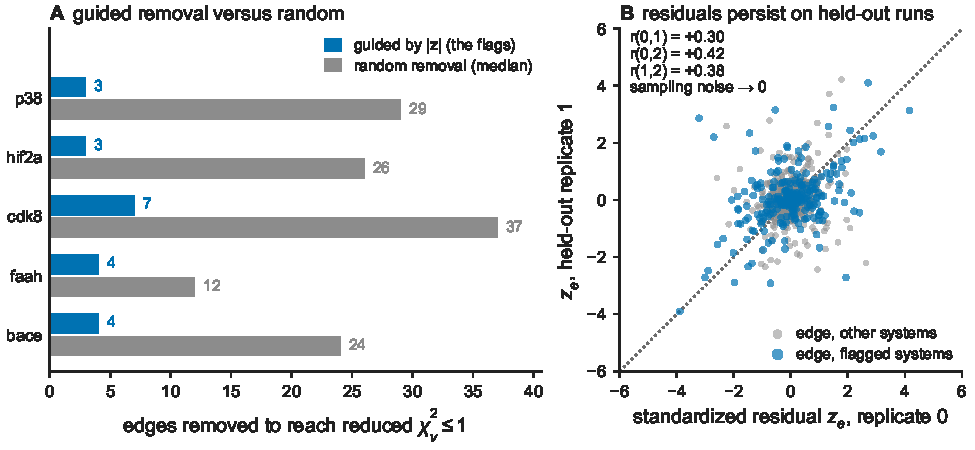
\includegraphics[width=0.92\textwidth]{figL_validation.pdf}
\caption{\textbf{Edge-removal repair test and cross-replicate residual reproduction.} (A)
Number of edges removed, in descending order of $|z|$, before reduced $\chi^2\le1$ is
restored: guided removal of the flagged high-$|z|$ edges versus random removal, per system.
(B) Standardized residual $z_e$ from a replicate-0 network fit versus $z_e$ from a
replicate-1 fit, for edges in flagged and in non-flagged systems, with the $y=x$ line and
the Pearson correlation between each pair of replicates.}
\label{fig:Lval}
\end{figure}

\begin{figure}[t]\centering
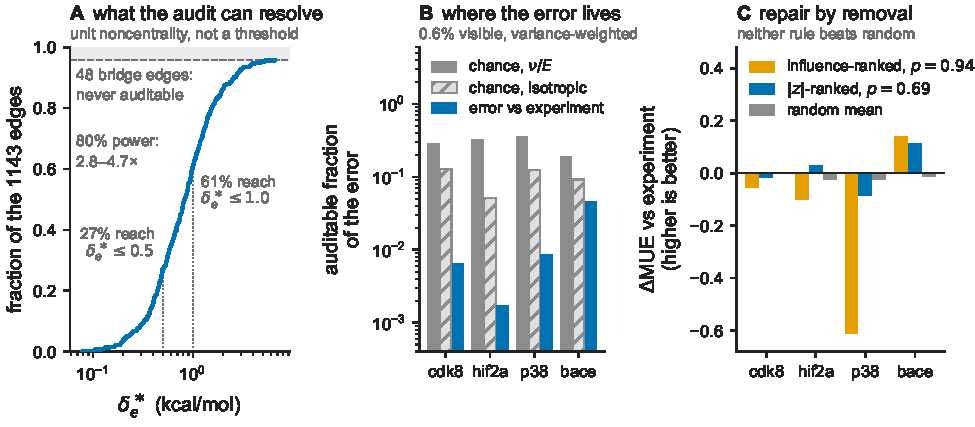
\includegraphics[width=\textwidth]{figHodge_where_the_error_lives.pdf}
\caption{\textbf{What the audit covers, and what the error does.} (A) Cumulative fraction of the
$1143$ benchmark edges against the shift $\delta^\ast_e$ each could detect, with the bridge edges
marked as the ceiling they impose. (B) Fraction of a system's error against experiment lying in the
auditable subspace, against the fraction an error field with no preferential alignment would show,
on the four systems with public affinities. (C) Change in mean unsigned error against experiment
after removing the same number of edges chosen by influence, by standardized residual, and at
random.}
\label{fig:Hodge}
\end{figure}

\subsection{Where the error is, and why removing edges cannot reach it}\label{sec:hodge}
Theorem~\ref{thm:hodge} makes two quantities measurable that were previously matters of
assumption: how much of a network is auditable at all, and how much of its real error the audit
can reach. Both are answered on this benchmark in Figure~\ref{fig:Hodge}.

Of the $1143$ edge dimensions carried by the $48$ systems with a cycle, $372$ lie in the cycle
space. Two-thirds of the error space is node-consistent and therefore invisible to every
closure-based diagnostic, this one included. Forty-eight edges are bridges, carrying no evidence
at any magnitude. Half the remaining edges cannot resolve a shift below $0.79$ kcal/mol, and only
$27\%$ of all $1143$ can resolve one of $0.5$; the detectable-shift resolution of the median edge is the size of
the error the field is trying to find (Figure~\ref{fig:Hodge}A).

That is the capacity of the audit. Its reach on real error is smaller. On the four systems grounded
against experiment below, the fraction of the measured error against experiment that lies in the
auditable subspace is $0.6\%$ pooled, and between four and $187$ times below the $\mathrm{dof}/E$
level an unaligned error field would show (Figure~\ref{fig:Hodge}B). Two properties of the
measurement keep it from being an artefact. It is a near-identity rather than a fit: experimental
affinities are per-ligand, so the experimental $\ddG$ vector is a gradient field, $\Pi\varepsilon$
reduces to the closure residual, and the visible fraction is the closure statistic divided by the
total squared standardized error. And it survives the obvious contaminants: recomputing it on
medians rather than sums moves it to $0.15$--$0.68\%$, so it is not carried by a few large
residuals, and \texttt{bace}, whose ligand set contains no enantiomer pair collapsed by the
stereo-blind affinity join, shows it as plainly as the rest. Per-edge error against experiment runs
$1.06$--$1.45$ kcal/mol at the median against reported standard errors of $0.14$--$0.40$: these
networks are wrong by several standard errors while closing their cycles, in the one direction
closure cannot look. What the design does not license is attribution. Experimental measurement
error and the annotation join are per-ligand, hence gradient fields too, so what is established is
that the dominant part of the error is node-consistent, not that it is force-field bias.

On \texttt{eg5}, whose ligands
carry ChEMBL identifiers, the network $\ddG$ (from the same GLS fit) agrees with real KIF11
experimental affinity~\citep{zdrazil2024chembl} at a mean unsigned error (MUE) of $0.79$ kcal/mol ($95\%$ bootstrap CI
$[0.59,0.97]$, conditional on the fitted network; Pearson $R=0.65$ $[0.30,0.83]$, $p{\approx}2{\times}10^{-4}$, $n=28$), and its clean cycle-closure reduced
$\chi^2=0.64$ is consistent: a QC-clean system is
indeed accurate. Acting on the QC does \emph{not} improve accuracy here (internal $|z|$ vs
error-against-experiment: $r=+0.13$), exactly as the scope predicts: on a clean system the
residual error against experiment is dominated by node-consistent force-field bias, which cycle
closure cannot see. The complementary test, that repairing a \emph{flagged} system improves its
accuracy, needs experimental affinities for the flagged systems; these are not directly tabulated
in the replicate set but are recoverable by per-paper ChEMBL structure-search. Of
the six flagged systems, four clear a $60\%$ public-ChEMBL coverage gate (\texttt{cdk8, hif2a, p38,
bace}; connectivity-based structure matching, one assay per system, IC50 before Ki, never mixed);
their baseline network MUE against this grounded experimental affinity is $0.79$--$1.47$ kcal/mol,
typical-magnitude FEP error, confirming the grounding itself is sound. On these four, guided
removal of the flagged high-$|z|$ edges (the same repair order as Figure~\ref{fig:Lval}A, fixing a
removal count $K=1$--$3$ per system) does \emph{not} reduce MUE-vs-experiment more than an
equal-size random removal (Supplementary Figure~\ref{fig:Lcausal}; per-system one-sided permutation
$p=0.905,0.136,0.880,0.071$; combined Stouffer $p=0.48$, sign test $p=0.69$, pre-registered success
required Stouffer $p<0.05$): two systems improve slightly over their random-null mean and two
worsen slightly, a wash with no system individually significant. The remaining two flagged systems
(\texttt{brd4, faah}) did not clear the coverage gate and are not included.

That null is what Theorem~\ref{thm:hodge} predicts and what the paragraph above measures. A removal
rule reads the visible part of the error; the visible part carries under one per cent of what is
wrong with these networks, and by part (ii) it is the part that biases the fitted potentials least.
A pre-registered second rule confirms the reading and rules out the obvious escape, that the
ranking was simply the wrong one. Part (ii) suggests ranking edges by influence rather than by
residual, $|z_e|\sqrt{(1-h_e)/h_e}$, the classical form that weights an edge by the bias its error
induces instead of by its visibility. At the same removal counts it performs worse than the rule it
was meant to replace (Stouffer $p=1.00$ against $0.48$; better on one system of four; paired sign
$p=0.94$; Figure~\ref{fig:Hodge}C). The reason is the same measurement: the influence form divides a
residual by a small curl-leverage to recover the error of a single anomalous edge, and a smooth
per-ligand field is not concentrated on any edge, so the division returns amplified noise.

The consequence for practice is a change of use rather than an abandonment. A flag remains a
system-level signal that a protocol has produced results inconsistent beyond sampling, and that
signal reproduces across replicates. It is not a repair target: deleting the edges it names cannot
recover accuracy against experiment, because accuracy against experiment is set by a component the
audit is blind to by construction. Reaching that component needs information from outside the
network, and by part (iv) the arithmetic of doing so with absolute measurements is unforgiving:
one anchor per component fixes only an arbitrary offset, and every dimension after that costs one
more measured ligand.

\paragraph{Summary.} The calibrated bar supplies, for free, the null model that turns FEP
cycle-closure into a quality-control test separating reproducible from sampling inconsistency on
real networks, whose output reproduces on replicates it never saw and which a bar as overconfident
as the learned $\sigma$ measured here destroys. Theorem~\ref{thm:hodge} bounds what that test, or
any other of its kind, can be asked for: it reads a third of the error space and, on the systems
where the comparison can be made, under one per cent of the error. The bound is the reason the
instrument is worth calibrating and the reason its flags are not a repair list.

\subsection{What survives a second replicate}\label{sec:stability}
The benchmark ships three independent repeats, so the flag set can be recomputed rather than
assumed. It does not hold up as a set. The same pipeline at the same FDR level returns
$\{$\texttt{bace}, \texttt{brd4}, \texttt{cdk8}, \texttt{faah}, \texttt{hif2a}, \texttt{p38}$\}$ on
the first replicate, $\{$\texttt{bace}, \texttt{brd4}, \texttt{ciordia\_retro}, \texttt{hif2a},
\texttt{p38}, \texttt{renin}$\}$ on the second and $\{$\texttt{bace}, \texttt{cdk8},
\texttt{renin}$\}$ on the third: eight systems are flagged at least once, one
(\texttt{bace}) is flagged every time, and pairwise Jaccard overlap is $0.50$, $0.29$, $0.29$
against $0.056$ for size-matched random draws, averaged over the three pairs. The churn is not a threshold artefact and
persists from $\alpha=0.01$ to $\alpha=0.20$ (Supplementary Figure~\ref{fig:Stab}). Pooling the
three replicates flags seven systems, the union minus \texttt{faah}.

The churn is not explained by how cyclic the networks are. Cycle counts on this benchmark are
low: nine of the $48$ systems carry exactly one independent cycle, twenty-three carry three or
fewer, and the quartiles are $2$, $5$ and $12$. A reduced $\chi^2$ on one or two degrees of freedom
is an unstable statistic, and those systems do swing more across repeats. But they are not the
systems that move in and out of the flag set: seven of the eight ever flagged are well connected,
and restricting the comparison to the best-connected third of the benchmark leaves the pairwise
overlap no better than it is over all $48$. The instability sits where the test has power, which
makes it a property of the measurement rather than of thin networks.

Two things do survive. The ranking of systems by closure inconsistency reproduces across
replicates (Spearman $0.649$, $0.644$, $0.723$ over all $48$ systems), and the dependence of
selectivity on $\sigma$-calibration, which is the claim this section is actually making, is
essentially unmoved: the $\times0.15$ shrink flags $42$, $41$, $41$ systems, the calibrated bar
$6$, $6$, $3$, a $\times1.3$ inflation $1$, $1$, $1$, and a $\times2$ inflation none, on the three
replicates respectively. What a single replicate supports is a ranking and a calibrated operating
point, not a list of names. Among the published six, \texttt{faah} is the weakest on every
measure: its reduced $\chi^2$ crosses one in both directions across replicates
($3.71$, $0.45$, $1.47$), its standardized residuals barely reproduce between replicates
($r=-0.085$), and it is the one member the pooled fit drops.

\subsection{Out-of-sample behaviour}\label{sec:oos}
Two checks use one replicate to predict another and so cannot be circular. First, the per-edge
miscalibration measured from replicates two and three predicts the closure statistic of the
replicate they exclude: with $V_e^{\mathrm{rep}}=c_e^2V_e^{\mathrm{true}}$ as above,
Theorem~\ref{thm:cons} makes
$\mathbb{E}[\chi^2_\nu]$ the curl-leverage-weighted mean of $c_e^{-2}$, and that prediction
correlates with the observed per-system $\chi^2_\nu$ at Spearman $0.648$ ($n=48$). Both sides divide by the same reported variance, so the reference is not zero: under a simulation with no systematic error anywhere the same statistic returns $0.059$ with a $95\%$ upper limit of $0.364$, and $0.648$ exceeds every one of $200$ draws (Supplementary Figure~\ref{fig:OOS}A). The aggregate level agrees less well: the predicted $\mathbb{E}[\chi^2_\nu]=0.85$ $[0.63,1.08]$ sits below the observed degree-of-freedom-weighted value of $1.32$ $[0.81,1.80]$, and the two intervals overlap without the prediction covering the observation. What this establishes is narrower than it first reads. The prediction is built entirely from
measured miscalibration, so a rank agreement of this size says that the closure statistic largely
reads out how well each system's bars are scaled. It is a statement about what the test responds
to, not evidence that the flagged systems are in error. The flagged systems do sit \emph{above}
the line, which is what any reproducible offset does: it inflates a closure residual without
inflating the spread between repeats. Being reproducible across repeats that share a
starting structure is what places a system above the line, and that is weaker than being in error.

Second, edges selected on one replicate are more inconsistent on the two held out than
equal-size random selections are (mean gain in held-out reduced $\chi^2$, Stouffer
$p=1.3\times10^{-3}$, $1.3\times10^{-3}$, $4.4\times10^{-3}$ over the three rotations), while a
topology-only control built from curl-leverage is indistinguishable from random
($p=0.21$--$0.91$). We calibrated each candidate statistic against a no-error null before using
it and report the realized level of all of them, including the two we discarded for firing far
above nominal. Only the consistency-gain statistic is specific to the flagged systems: an
$|z|$-rank-matched control drawn from unflagged systems reproduces the leverage-normalised
residual signal but not the consistency gain. The effect is an aggregate one, significant
individually in two of the five testable systems.

\section{An applicability map: where this calibration helps, and where it does not}\label{sec:audit}
The detector of Section~\ref{sec:qc} is a real-data payoff; whether the same free calibration
improves downstream machine learning is a separate question, and mostly it does not. These
negatives are the reason to believe the positive result. Six tasks are audited, four for
performance and two for decision quality, and Supplementary Table~\ref{tab:audit} collects every
effect against its baseline. Three performance tasks, interval sharpness, commit-to-synthesis
selection and reward re-ranking over a measured congeneric set, run with the commit-trust decision
task on the public OpenFF protein--ligand benchmark~\citep{hahn2022plbench} (FEP+ and Merck
data~\citep{wang2015fep,schindler2020merck}, experimental $\ddG$ labels, both-endpoint
scaffold-disjoint out-of-distribution splits); edge ranking in active learning and the stopping
decision run in controlled simulations. The amortized $\sigma$ under test is the trunk's
predictive uncertainty on unseen $\ddG$,
$\sigma_{\text{total}}=\gamma\sqrt{\sigma^2_{\text{ens}}+\sigma^2_{\text{ale}}}$: deep-ensemble
epistemic spread and benchmark aleatoric floor, conformally scaled at miscoverage $\alpha=0.1$. It
is not Figure~\ref{fig:A}'s per-edge BAR sampling-se or its learned foil; a bare ``$\sigma$'' below
means $\sigma_{\text{total}}$.

\paragraph{Trust, where it pays.} Fixing the ensemble mean and varying only the uncertainty in a
commit rule (commit iff the lower-confidence bound $\mu-\kappa\sigma\ge\tau$), an overconfident
epistemic-only $\sigma$ over-claims badly: its realized-versus-claimed correctness shortfall is
$+0.182$ $[0.132,0.225]$ larger than the decomposed $\sigma$'s, which is calibrated-to-conservative
(Supplementary Figure~\ref{fig:J}B). The trust is not unique to the physics $\sigma$: temperature
scaling~\citep{guo2017calibration} or split-conformal recalibration of the same overconfident
$\sigma$ recovers it (both differences from ours indistinguishable from zero). Trustworthy
decisions need \emph{some} proper calibration; the physics $\sigma$ supplies it at no
calibration-set cost for the aleatoric term. The same lesson appears in a controlled
active-learning simulation, where a calibrated learner's claimed confidence tracks actual top-$k$
correctness ($|\Delta|=0.022$) and stops at $30$ calls $82\%$ correct, while an overconfident one,
its assumed posterior se scaled by the $0.15\times$ measured in Figure~\ref{fig:A}, stops twice as
early at only $60\%$ correct (Supplementary Figure~\ref{fig:G}).

\paragraph{Sharpness, ranking and selection, where it does not.} On real held-out trunk residuals
at matched $\sim$$0.90$ marginal coverage the decomposed interval is slightly \emph{wider} than
flat split-conformal (width ratio $0.92\times$), because epistemic spread is small against the
large irreducible out-of-distribution error; its conditional calibration is comparable to a fair
Mondrian-by-target conformal and the advantage is not significant (ours$-$split $-0.044$
$[-0.121,0.005]$; Supplementary Figure~\ref{fig:Breal}). The supplement's synthetic illustration,
whose generative structure the decomposition knows, is up to $2.2\times$ sharper than
split-conformal; that does not transfer. For edge ranking, sandwich against naive weights differ by
$0.98\times$ $[0.93,1.03]$ on calls-to-top-$k$: in a connected graph the GLS contrast mean is
unbiased for \emph{any} positive weights, so the weight value is second-order for ranking. So too
for commit selection at matched volume, where the $\sigma$-aware ranking does not beat a raw-$\mu$
ranking ($-0.006$ $[-0.016,0.007]$). A calibrated bar says \emph{whether} to act, not \emph{which}
action ranks first.

\paragraph{Reward re-ranking, where it hurts.} A trajectory-balance
GFlowNet~\citep{bengio2021gflownet,malkin2022tb} samples a held-out target's measured congeneric
series under three rewards. On \texttt{eg5}, the on-disk target with the largest $\sigma$ spread and
so the one where a calibrated reward genuinely re-ranks candidates, the calibrated lower bound
\emph{lowers} the true hit-rate ($0.140$ against raw $0.249$; cal$-$raw $-0.109$
$[-0.150,-0.072]$; Supplementary Figure~\ref{fig:K}). The high-$\sigma$ ligands are the chemically
novel \emph{strong} binders ($\mathrm{corr}(\sigma_{\text{total}},\text{affinity})=+0.42$), so the
penalty $-\kappa\sigma$ demotes the true winners. Resting on one evaluable target this is a
hypothesis rather than a transferable diagnostic: where $\sigma$ flags novelty rather than quality,
an uncalibrated reward is safer.

\paragraph{Synthesis.} A calibrated per-edge $\sigma$ does not sharpen intervals on real data, does
not re-rank what to compute or what to commit, and does not steer reward re-ranking toward better
molecules on the one evaluable congeneric set; it pays on commit trust and on stopping in
simulations that do not consume the physics variance; and an \emph{overconfident} $\sigma$ silently
corrupts the stop and commit decisions. Calibration is a trust and decision instrument, not a
performance multiplier. The graph weight earns its place through \emph{structure} rather than
magnitude: it makes the gauge directions exactly unidentifiable, and by Gauss--Markov its numerical
value does not improve ranking.

\section{Computational details}\label{sec:methods}
\paragraph{Data.} The controlled panel of Figure~\ref{fig:A} uses the \texttt{alchemtest} BACE1
relative-binding and benzene sets, from which forward and reverse work samples are available per
$\lambda$ window. The replicate validation, the cycle-closure test and every experiment on real
binding data use the OpenFE IndustryBenchmarks2024 release~\citep{baumann2025industrybenchmarks},
which ships three independent protocol repeats per transformation: $1145$ edges across $49$
benchmark systems. A system here is one of the benchmark's named edge networks and not one
protein: \texttt{jak2\_set1} and \texttt{jak2\_set2}, and \texttt{hsp90\_single\_ring} and
\texttt{hsp90\_kung}, are separate systems built on the same protein, so the system count exceeds
the number of distinct proteins. The
$48$ systems with at least one independent cycle, which between them hold $1143$ of the $1145$
edges, admit the closure test, and each counts as one hypothesis in the Benjamini--Hochberg
correction; the single remaining system is acyclic and contributes the other two edges. The
per-system calibration ratios of Figure~\ref{fig:Arep}B are pooled instead over the $34$ systems
that carry at least eight edges, eight being the smallest edge count at which a ratio pooled
against an $n=3$ replicate spread is stable enough to plot on its own row; the other fifteen
systems enter the aggregate ratio and the per-edge panel but are not shown individually. Grounding
against measured affinity uses public ChEMBL $\mathrm{IC}_{50}$ values. No free-energy simulation
was run for this work; all alchemical output is taken as published.

\paragraph{Per-edge variance.} $\dFh$ is obtained by solving Bennett's estimating equation
$S(\Delta F)=0$ by scalar root-find, and its variance from the closed form $B/I^2$ of
Theorem~\ref{thm:sand} evaluated at the root. The backward pass uses the implicit function
theorem, $\partial\dFh/\partial\theta=(1/I)\,\partial_\theta S$, so it costs one division and does
not unroll the root-find; gradients are checked against finite differences to machine precision.

\paragraph{Cycle-closure test.} Node potentials are fitted by generalized least squares on the
signed incidence matrix of the perturbation network, whitened by the per-edge standard errors, so
that the fit is a weighted least-squares problem with conductances $1/V_e^{\mathrm{rep}}$. Writing $N$ for that incidence matrix, to keep $B$ for the sandwich meat of
Theorem~\ref{thm:sand}, the statistic is the reduced $\chi^2$ of the residuals with
$\mathrm{dof}=E-\operatorname{rank}(N)$; per-system tail
probabilities use the exact regularized upper incomplete gamma function rather than a
Wilson--Hilferty approximation, and systems are flagged by Benjamini--Hochberg control of the
false discovery rate at $\alpha=0.05$ across systems. The population for the closure test is the
$48$ systems that carry at least three replicate-$0$ edges and at least one independent cycle,
which between them hold $1143$ of the benchmark's $1145$ edges.

\paragraph{Simulation protocols.} Two protocols underwrite numbers quoted above: the pure-null
simulation that supplies every realized false-flag level, and the reproducible-systematic magnitude
used as the label in detection comparisons. Both are specified in the Supporting Information.

\paragraph{Model architectures.} The amortized predictor used in the acquisition, stopping and
reward experiments and the learned-variance foil of Figure~\ref{fig:A} are separate and much
smaller models; their features, layer sizes, objectives and training budgets are specified in the
Supporting Information.

\paragraph{Software.} Python $\geq3.11$ with numpy $2.5.0$, scipy $1.18.0$, pymbar $4.0.3$, torch
$2.12.1$, RDKit $2026.3.3$ and matplotlib $3.11.0$. The pipeline is deterministic: in the
environment recorded here, re-running a figure's command reproduces that figure's rendered raster
byte for byte, and this was checked on the figures that depend on ensemble training rather than
assumed. Their reproducibility has a stated cause. Ensemble training runs on CPU, full batch, for
a fixed number of epochs; each of the eight members takes its weight initialization and its
bootstrap resample from its own member index as the seed; and the ligand ordering that reaches the
featurizer and the sampler is sorted rather than read out of a set, so it does not depend on the
process-level string hash. Nothing in the training path is left to an unrecorded source of
variation.

\section{Limitations}\label{sec:limitations}
The sandwich is aleatoric-only and conditional on correctly sampled ensembles. Systematic
force-field bias lies outside it, and the out-of-distribution behaviour audited here rests on an
ensemble plus a scalar aleatoric floor: there is no learned force-field-correction head, so the
three-way decomposition of the synthetic illustration is not reproduced on real data.

The binding-edge se is validated against three independent replicates (Figure~\ref{fig:Arep}). In
aggregate it is conservative by $\sim$$1.41\times$, but calibration is heterogeneous: of the $34$
systems carrying at least eight edges, $28$ are conservative and six overconfident, namely
\texttt{t4\_lysozyme} $0.99\times$, \texttt{hif2a} and \texttt{bace} $0.96\times$, \texttt{faah}
$0.90\times$, \texttt{brd4} $0.76\times$, and the protonation variant
\texttt{bace\_p3\_arg368\_in} $0.41\times$, the only one of the six that is not marginal. Those
replicates are seed and velocity repeats from identical starting coordinates, so the
across-replicate SD is a lower bound on full reproducibility, excluding pose and preparation
variance, and the measured conservatism may be closer to neutral against real reproducibility.
The same restriction limits what the quality-control test can be said to detect. An inconsistency
reproducing across repeats that share one starting structure is more than sampling noise, but a
fixed consequence of that structure, a pose or a protonation assignment carried unchanged into all
three, would reproduce identically; the pooling argument of Figure~\ref{fig:L}C and the
cross-replicate residual correlation of Figure~\ref{fig:Lval}B are invariant to which of the two it
is, so the flags are reported as reproducible inconsistency throughout.

The test detects only \emph{edge-level} inconsistency, and neither removal rule improves accuracy
against experiment: guided removal ties random on the four grounded systems (Stouffer $p=0.48$;
Figure~\ref{fig:Lcausal}) and the influence rule does worse ($p=1.00$; Figure~\ref{fig:Hodge}C).
Theorem~\ref{thm:hodge} makes both nulls structural rather than underpowered and
Section~\ref{sec:hodge} measures the margin, but three restrictions attach to that measurement. It
rests on four systems, all of them flagged, so it characterises the systems the test selects rather
than the benchmark. It runs on a connectivity-based ChEMBL join, stereo-blind, so enantiomer pairs
sharing a 2D graph collapse to one experimental value, inflating absolute MUE while cancelling in
the guided-versus-random contrast since both arms read the identical cached affinity; the
experimental and annotation errors it carries are per-ligand quantities entering the same
unauditable subspace as force-field bias, so the measurement locates the error without attributing
it. And the influence rule is a second pre-registered hypothesis on the data that returned the
first null, reported as a second look rather than as independent confirmation. The theorem bounds
what a network's own edge values can support and says nothing against methods bringing information
from outside the network. A prospective flag, repair and remeasure test with new molecular
dynamics lies outside what public data can support.

The cross-replicate check shows that what is flagged reproduces across independent runs; it is not
a false-positive-rate guarantee and does not certify the nominal Benjamini--Hochberg rate. Recall
cannot be measured at all, there being no ground-truth error labels. Replacing each system's
reported standard error by its own replicate-measured calibration changes the flag set in both
directions and by an amount depending on the granularity: applied two-sided per edge the count goes
from six to seven, three systems entering and two leaving, and by each system's aggregate ratio to
sixteen with none leaving (Supplementary Figure~\ref{fig:Self}); applied one-sided, the direction
the circularity concern calls for, the per-edge arm retains two and the per-system arm all six
(Supplementary Table~\ref{tab:selfgrid}). Neither two-sided arm is false-discovery-rate controlled
at three replicates and no arm is reported as a flag set: under the pure-null simulation of
Section~\ref{sec:methods} their probability of at least one false flag is $0.59$ and $0.24$ against
the $0.04$ the uncorrected arm realizes at the same nominal level, and only the one-sided per-edge
arm holds it ($0.003$). What this establishes is that the flag set is sensitive to calibration
error of the size actually present, in both directions, which limits how far any single flag list
should be trusted.

Together with the median reduced $\chi^2$ of $0.34$, which implies limited single-replicate power,
that makes the flagged systems a floor rather than a prevalence estimate. \texttt{renin} carries
the reproducible signature by the pooled-replicate ratio, its reduced $\chi^2$ rising to $4.7$
pooled from a per-replicate mean of $2.5$, and clears the false-discovery threshold on two of the
three replicates though not on the first, which is the one the published list is drawn from; it is
a system that list misses rather than one the test misses, and \texttt{ciordia\_retro} is a second
such case. The error runs the other way too. \texttt{faah} clears the threshold on the first
replicate alone, its reduced $\chi^2$ crosses one in both directions across the three ($3.71$,
$0.45$, $1.47$), its standardized residuals essentially fail to reproduce between replicates
($r=-0.085$, the weakest of the eight systems ever flagged), and the pooled fit drops it, so we
report it as a flag a second replicate does not support rather than a member of the set on the
footing of \texttt{bace}, which is flagged on every replicate and by every criterion here.

The gauge-acquisition and stopping experiments are controlled simulations, and the reward
re-ranking audit rests on a single $\sigma$-varying target, so its conclusion that $\sigma$ tracks
novelty rather than quality is directional and should be tested across more chemotypes. The
amortized predictor carries a parity-odd readout channel because a geometric readout built only
from distances, norms or dot products is constant on an enantiomer pair; that requirement and the
completeness statement behind it are established in the Supporting Information, and nothing the
main text claims depends on them. Finally, a structure-based reverse screen on a separate
ten-target diverse-fold panel recovers the true target at top-$1$ $0.16$ (area under the curve
$0.62$) against $0.95$ ($0.99$) for the ligand-shape baseline of Supplementary
Figure~\ref{fig:F} and $0.10$ for random, raw docking scores not being comparable across pockets,
so the structure-directed regime is not claimed here.

\section{Conclusion}\label{sec:conclusion}
The error of a perturbation network splits in two, and the split is not a matter of degree. One
part lives in the cycles and can be audited; the other is a difference of per-ligand offsets and is
invisible to anything computed from the network's own numbers, at any magnitude. The two parts are
orthogonal complements, and the division falls in an awkward place: the part that biases the
answer is exactly the part that cannot be seen, and the part that can be seen biases nothing. On
the public benchmark examined here the auditable part spans a third of the error space, and on the
systems where the comparison against experiment can be made it carries under one per cent of what
is actually wrong.

That measurement fixes what the audit is for. Fitting a network's cycle closure against per-edge
precisions the estimator already reports turns a descriptive consistency check into a test with a
stated null, an operating point whose level can be measured, and an ordering of networks by how
far their own calculations disagree with each other. The same fit says before any simulation is
run which edges could carry evidence of an error and how large that error would have to be. What
the test does not deliver is a repair list: removing the edges it names does not recover accuracy
against experiment, and neither does removing the edges a rule built from the theorem itself
prefers. Closing the remaining gap requires information the network does not contain, and paying
for it in absolute measurements costs one ligand per dimension. Reading uncertainty off the physics
rather than learning it is what makes the audit free; knowing what the audit cannot reach is what
makes it honest.


\bibliography{refs}
\end{document}
